\chapter{Background estimation}\label{chap:Backgr}
\minitoc

 Main backgrounds for W analysis are coming from:
\begin{itemize}
\item Processes with $\tau$ leptons, misidentified as an electron or muon;
\item Leptonic Z-boson decays with one missreconstructed lepton;
\item QCD (or multijet) processes. In the electron channel the background is mostly jets faking electrons, while in the muon channel it consists of real muons produced in decays of mesons. %The $E_T^{miss}$ distribution is peaking
\end{itemize}
Most of the background processes are estimated using the MC simulation. In order to estimate the expected number of events, the simulated events are normalized to the cross-section predictions. Full list of simulated background samples together with the corresponding cross section predictions is shown in Tab.~\ref{tab:Backgrounds}. The multijet background is estimated using data driven method, as described below.


\begin{table}[!tbp]
    \caption{Background processes with their associated cross sections and uncertainties (if given) for $W\to l\nu$ and $Z\to ll$ processes. The quoted cross sections are used to normalize expected number of events.}
	\label{tab:Backgrounds}
	\begin{center}
		\begin{tabular}{c | c | c}
		\hline
		\hline
		Process & $\sigma \cdot BR $($\pm$unc.) [pb] & Order \\
\hline
$W^+ \to l \nu$ & \WPxsec ($\pm \WPxsecUncertanty$) & NNLO \\ 
$W^- \to l \nu$ & \WMxsec ($\pm \WMxsecUncertanty$) & NNLO \\ 
\hline
$Z \to ll$ & \Zxsec($\pm \ZxsecUncertanty$) & NNLO \\
\hline
$t \bar{t}$ & \Ttxsec & LO \\
$WW$ & \WWxsec & LO \\
$ZZ$ & \ZZxsec & LO \\
$WZ$ & \WZxsec & LO \\
\hline
\hline
\end{tabular}
\end{center}    
\end{table}

\section{Multijet background estimation}\label{sec:QCD}


The jet can fake the W-boson signature with single isolated lepton and large \etmiss in the event. Due to a large large theoretical uncertainties and high statistics needed, generation of MC simulation events for multijet background estimation becomes impractical. Instead data driven technique for multijet background estimation is used. In our case contribution from the multijet background  in the Z sample is negligible (Fig.~\ref{fig:CPMassZ}), so it is estimated just for \wenu and \wmunu processes. 

Data driven method allows to have model independent predictions with small statistical uncertainty. This method is using multijet enriched region, where signal events are suppressed. This is usually done by reversing identification or isolation criteria. It is assumed, that shape of the multijet background stays the same in the signal region. Normalization can  be derived in a control region through the template fit. 

This section describes method of multijet background determination, that have been used in 2.76 TeV data. 


\begin{figure}[!tbp]
\begin{minipage}[h]{0.49\linewidth}
\center{ 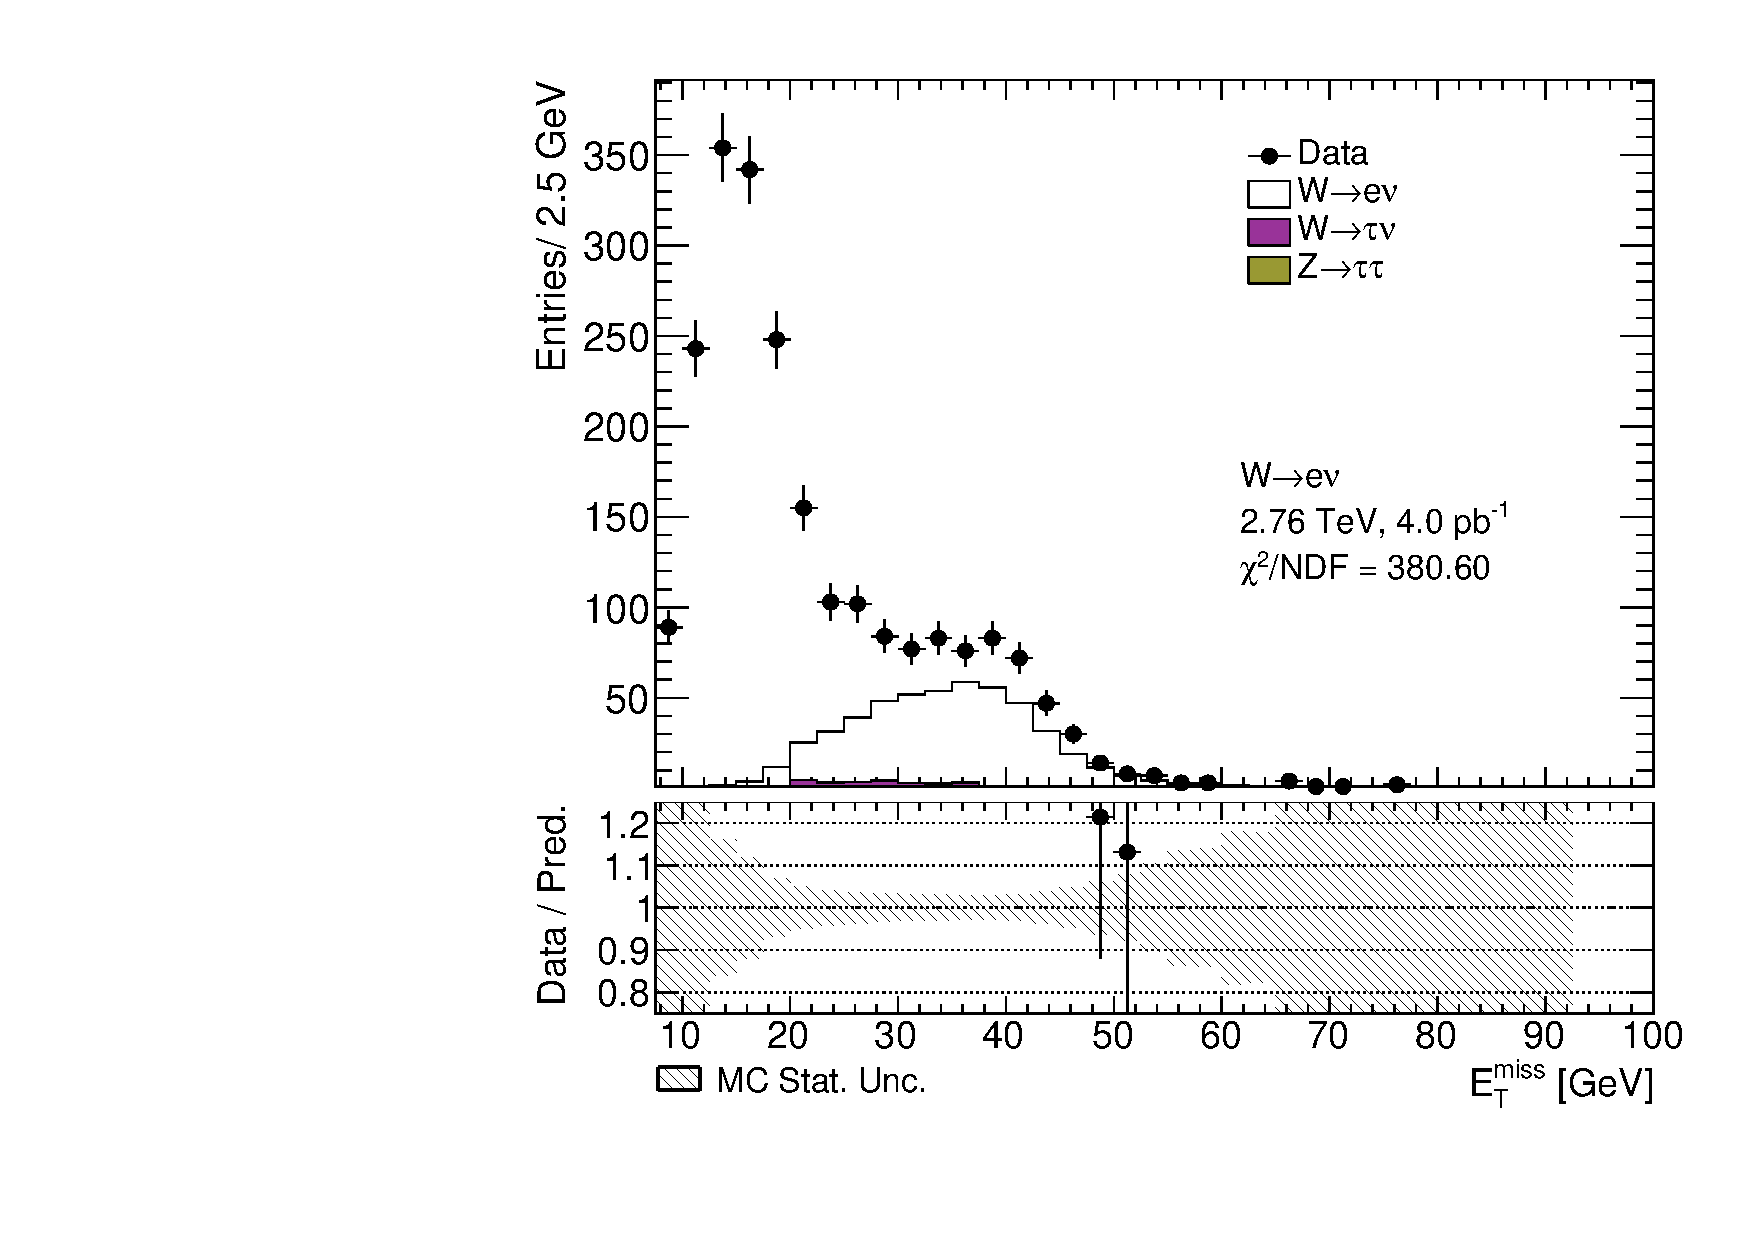
\includegraphics[width=1.\linewidth]{QCD/QCDetMissTempl.pdf} \\a)}
\end{minipage}
\hfill
\begin{minipage}[h]{0.49\linewidth}
\center{ 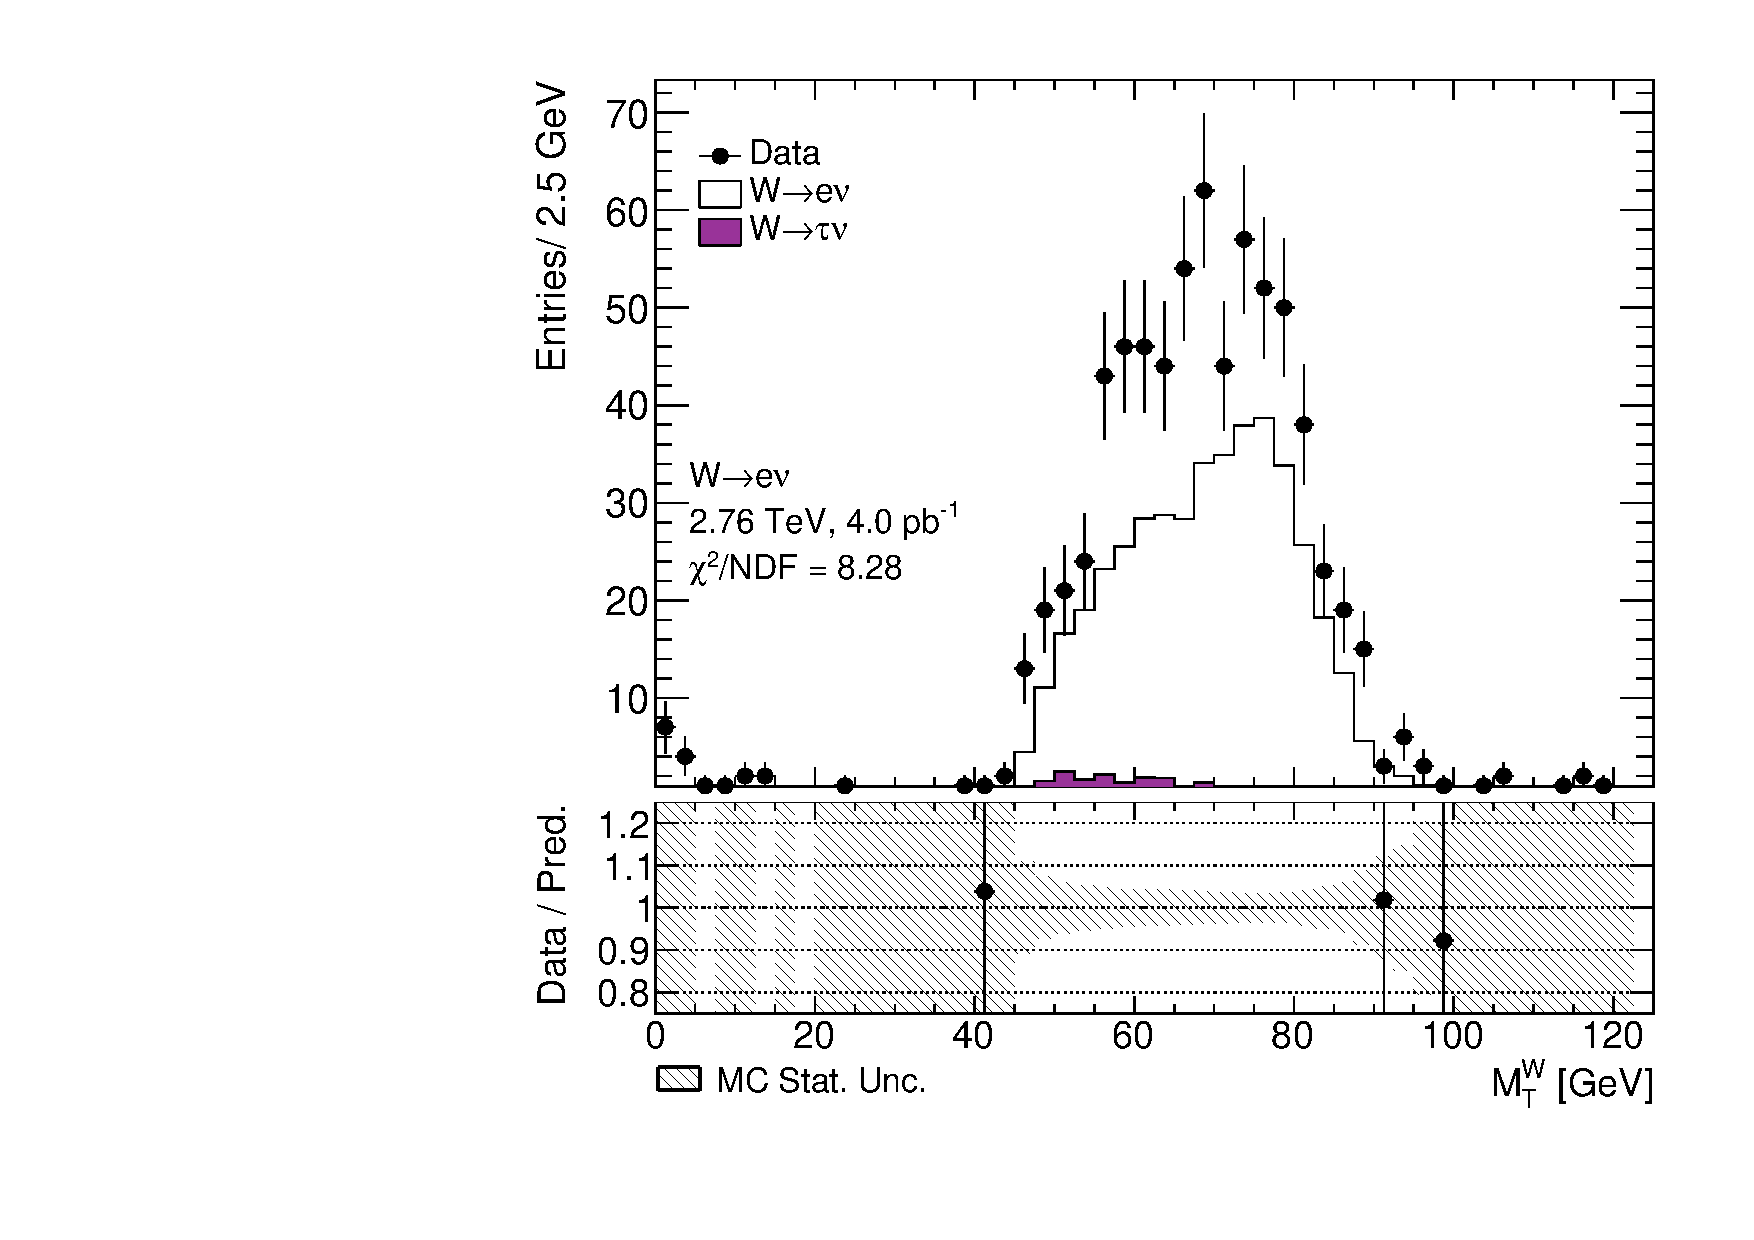
\includegraphics[width=1.\linewidth] {QCD/QCDmtWTempl.pdf} \\b)}
\end{minipage}
\caption{Distribution of a) missing transverse energy (\etmiss) and  b) transverse mass (\mtw) from the multijet template selection for \wenu candidate events.}
\label{ris:TemplateE}

\vfill

\begin{minipage}[h]{0.49\linewidth}
\center{ 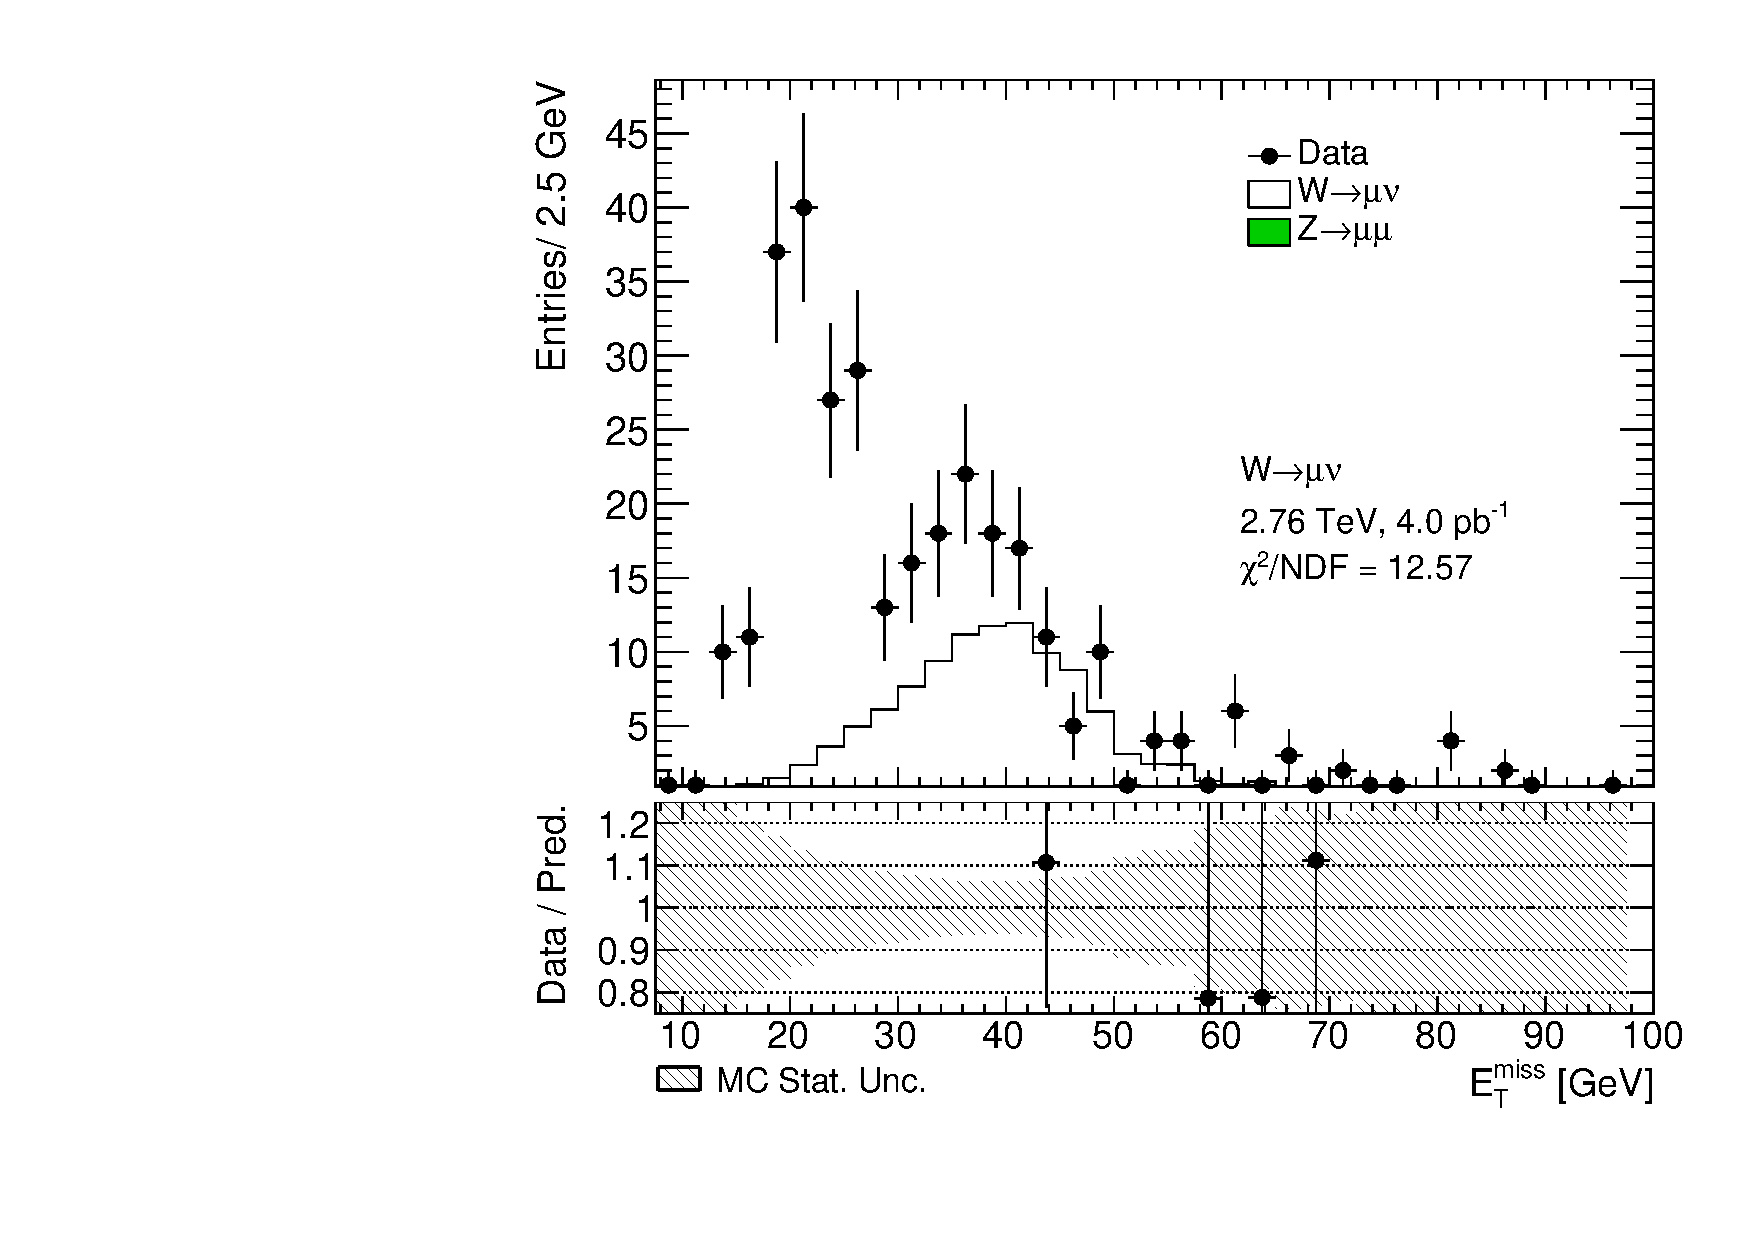
\includegraphics[width=1.\linewidth]{QCD/QCDWmuetMissTempl.pdf} \\a)}
\end{minipage}
\hfill
\begin{minipage}[h]{0.49\linewidth}
\center{ 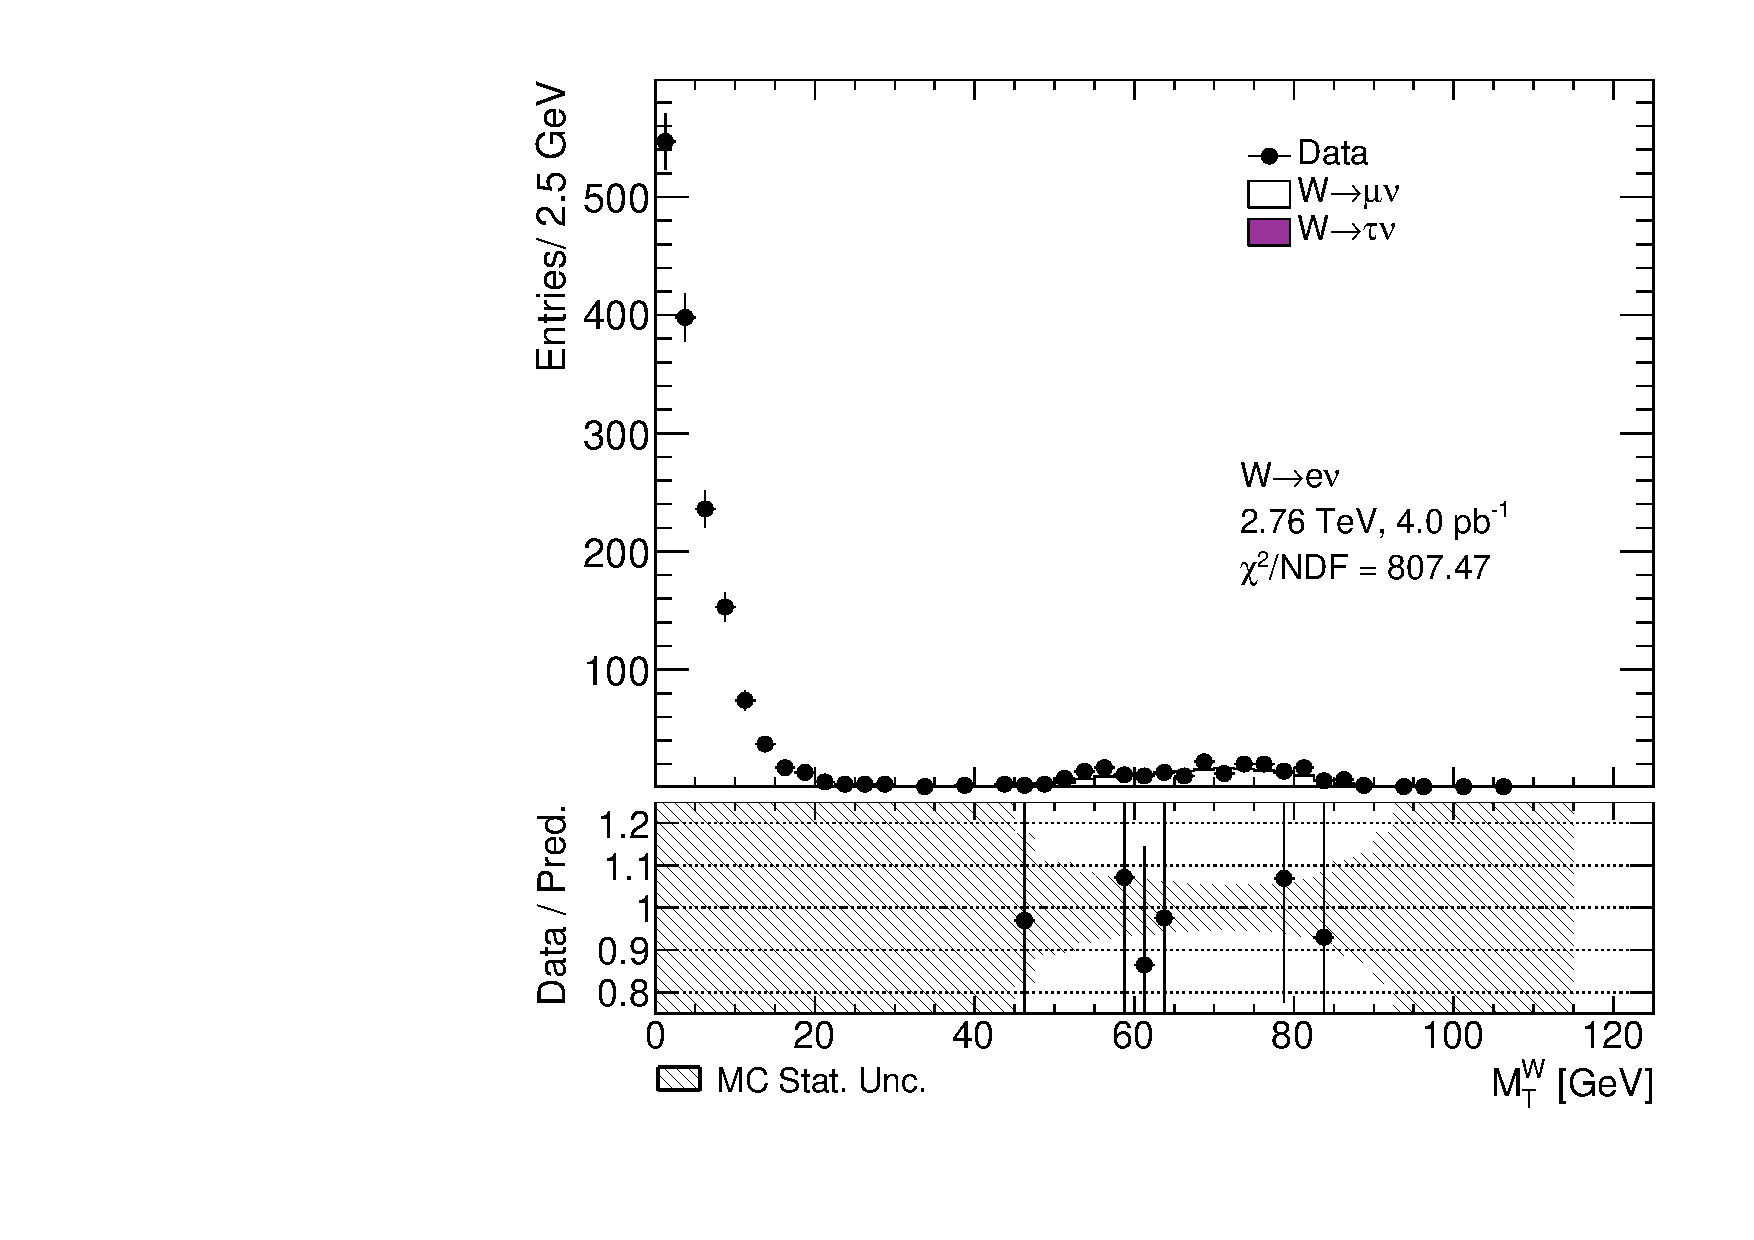
\includegraphics[width=1.\linewidth] {QCD/QCDWmumtWTempl.pdf} \\b)}
\end{minipage}
\caption{Distribution of a) missing transverse energy (\etmiss) and  b) transverse mass (\mtw) from the multijet template selection for \wmunu candidate events.}
\label{ris:TemplateMu}
\end{figure}

\subsection{Template selection}

A study have been performed to determine appropriate template selection. Because of the origin of the multijet background, missing transverse energy \etmiss should be smaller in background sample, than in a signal region. Releasing the \etmiss criteria allows to gain a bigger statistics for a multijet template. Another possibility is to relax the transverse mass \mtw requirement. Most of the multijet background events should contribute to the small \mtw region. The template sample can contain also contributions from other backgrounds (mostly coming from \wlnu). The best template selection should allow for big data statistics and small electroweak contributions at the same time. In order to suppress the signal additionally reversed ID or isolation criteria is applied. 

In electron channel, the template selection requires an electron candidate to fail medium identification criteria, but to pass loose selection. Control distributions for a different template selection in electron channel are shown in Fig.~\ref{ris:TemplateE}. Relaxed \etmiss criteria allows to gain bigger template statistics. 

In a muon channel template selection is build by inverting isolation criteria (\ptcone > 0.1). In case of \wmunu the multijet background template the best statistics is achieved by relaxing mass transverse \mtw requirement (Fig.~\ref{ris:TemplateMu}). 

In order to avoid double counting, electroweak processes (i.e. signal and backgrounds) are subtracted from a template. The total number of events in the template can be defined as:
\begin{equation}
N_{template} = N^{bkg\, enriched}_{data} - \sum_{j}^{MC} N_{MC_j}^{bkg\, enriched},
\end{equation}
where $N^{bkg enriched}_{data}$ and $N_{MC_j}^{bkg enriched}$ are numbers of the events in a background enriched sample in data and different MC samples respectively. The resulting template statistic is 1348 and 1509 events for \wenu and \wmunu respectively. 


\subsection{Methodology of the template sample normalization}

\begin{figure}[!tbp]
\begin{minipage}[h]{0.49\linewidth}
\center{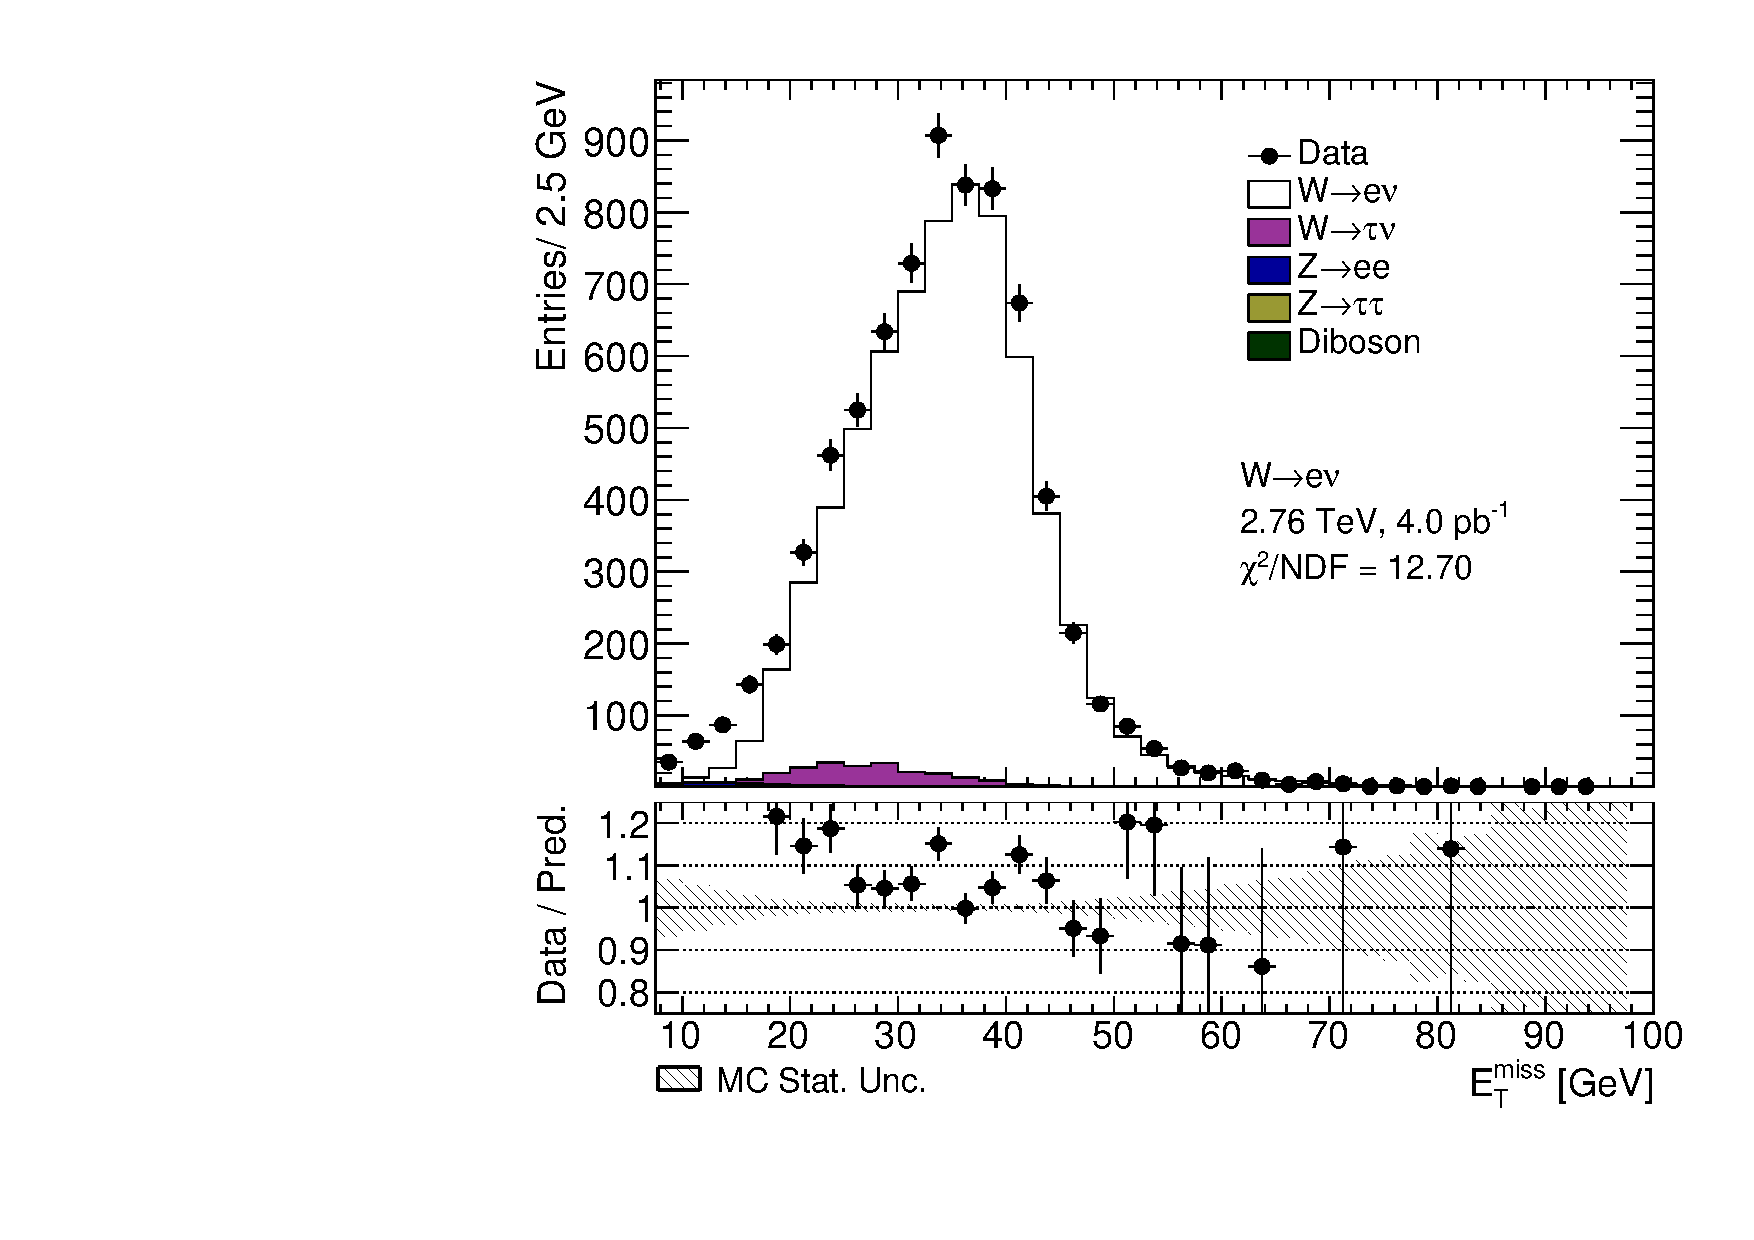
\includegraphics[width=1.\linewidth]{QCD/QCDetMissFit.pdf} \\ a)}
\end{minipage}
\hfill
\begin{minipage}[h]{0.49\linewidth}
\center{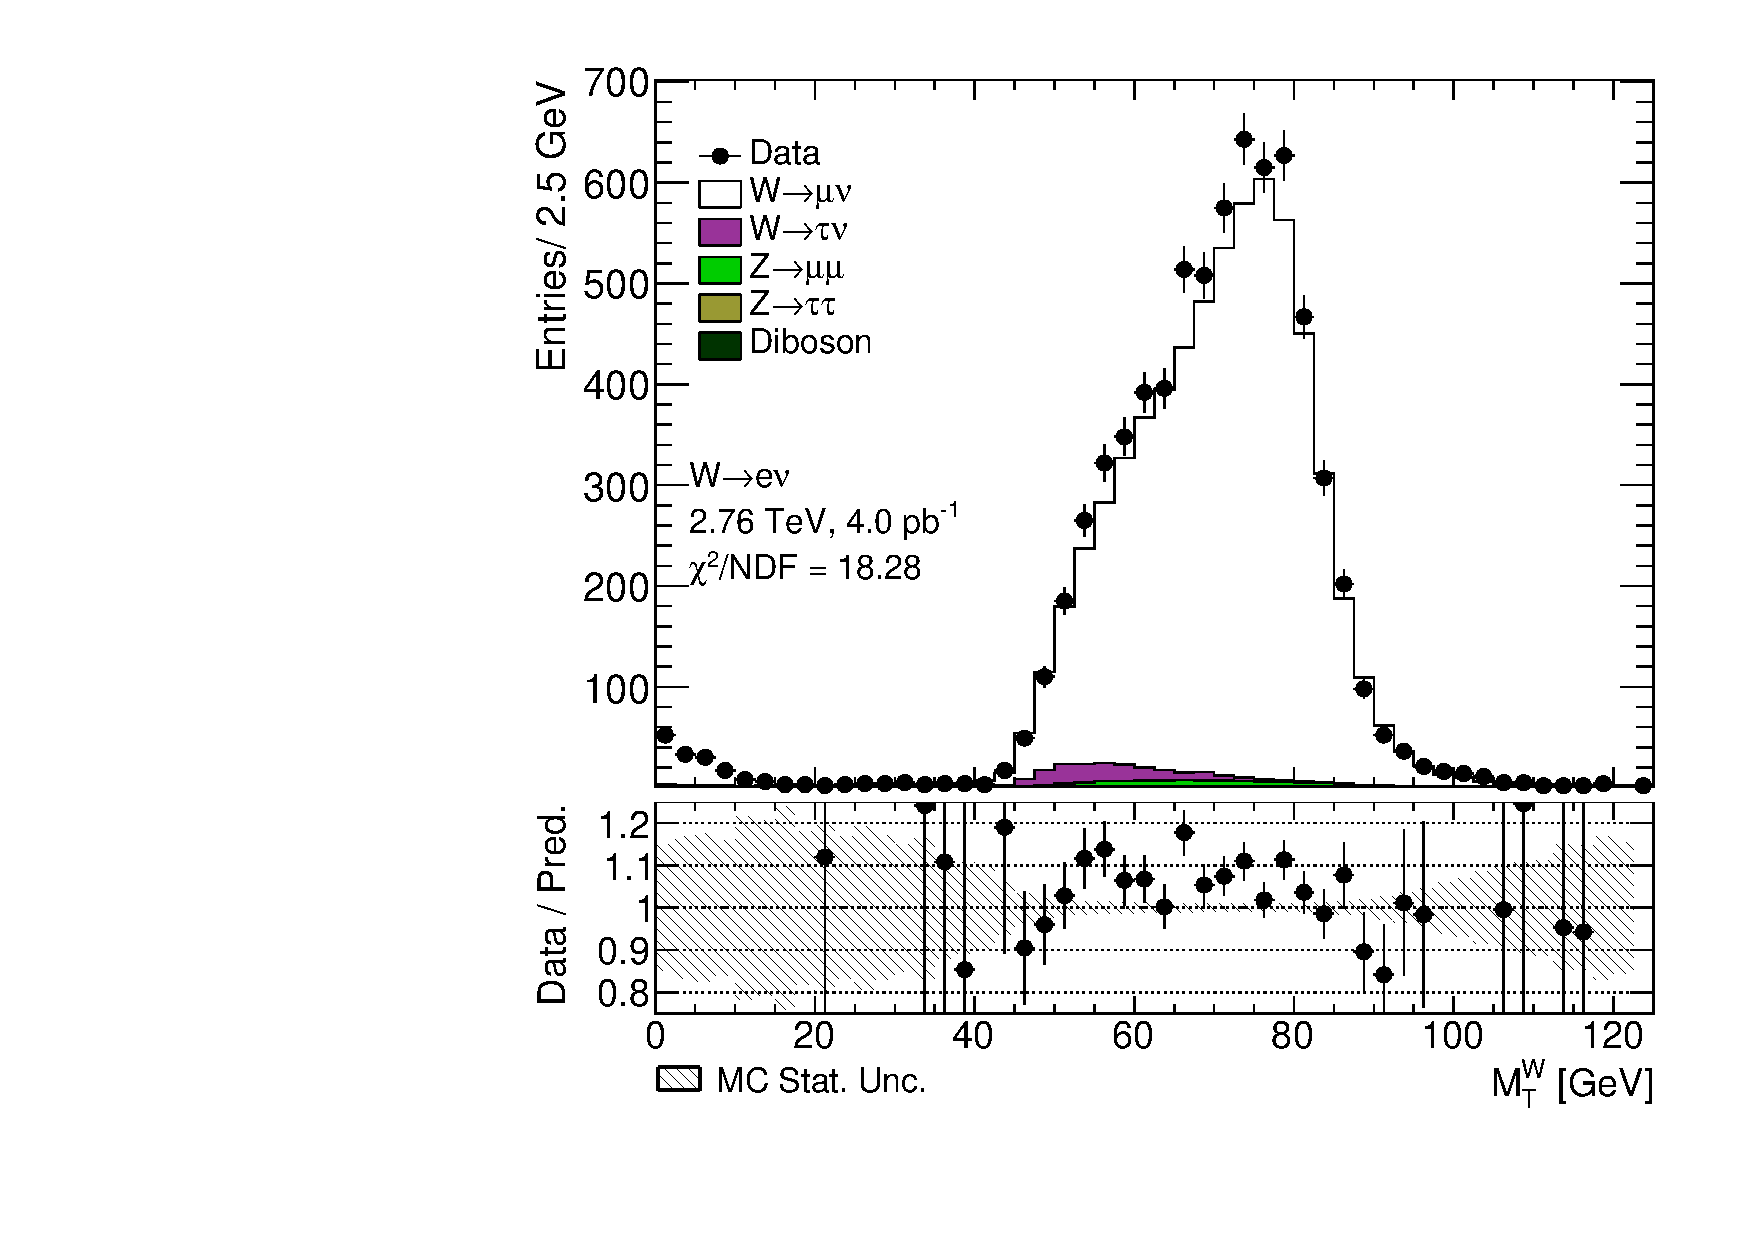
\includegraphics[width=1.\linewidth]{QCD/QCDWmumtWFit.pdf} \\ b)}
\end{minipage}
\caption{Distributions used for multijet background estimation for a) \wenu b) \wmunu.}
\label{ris:FitDistributions}
\end{figure}

\begin{figure}[!tbp]
\begin{minipage}[h]{0.49\linewidth}
\center{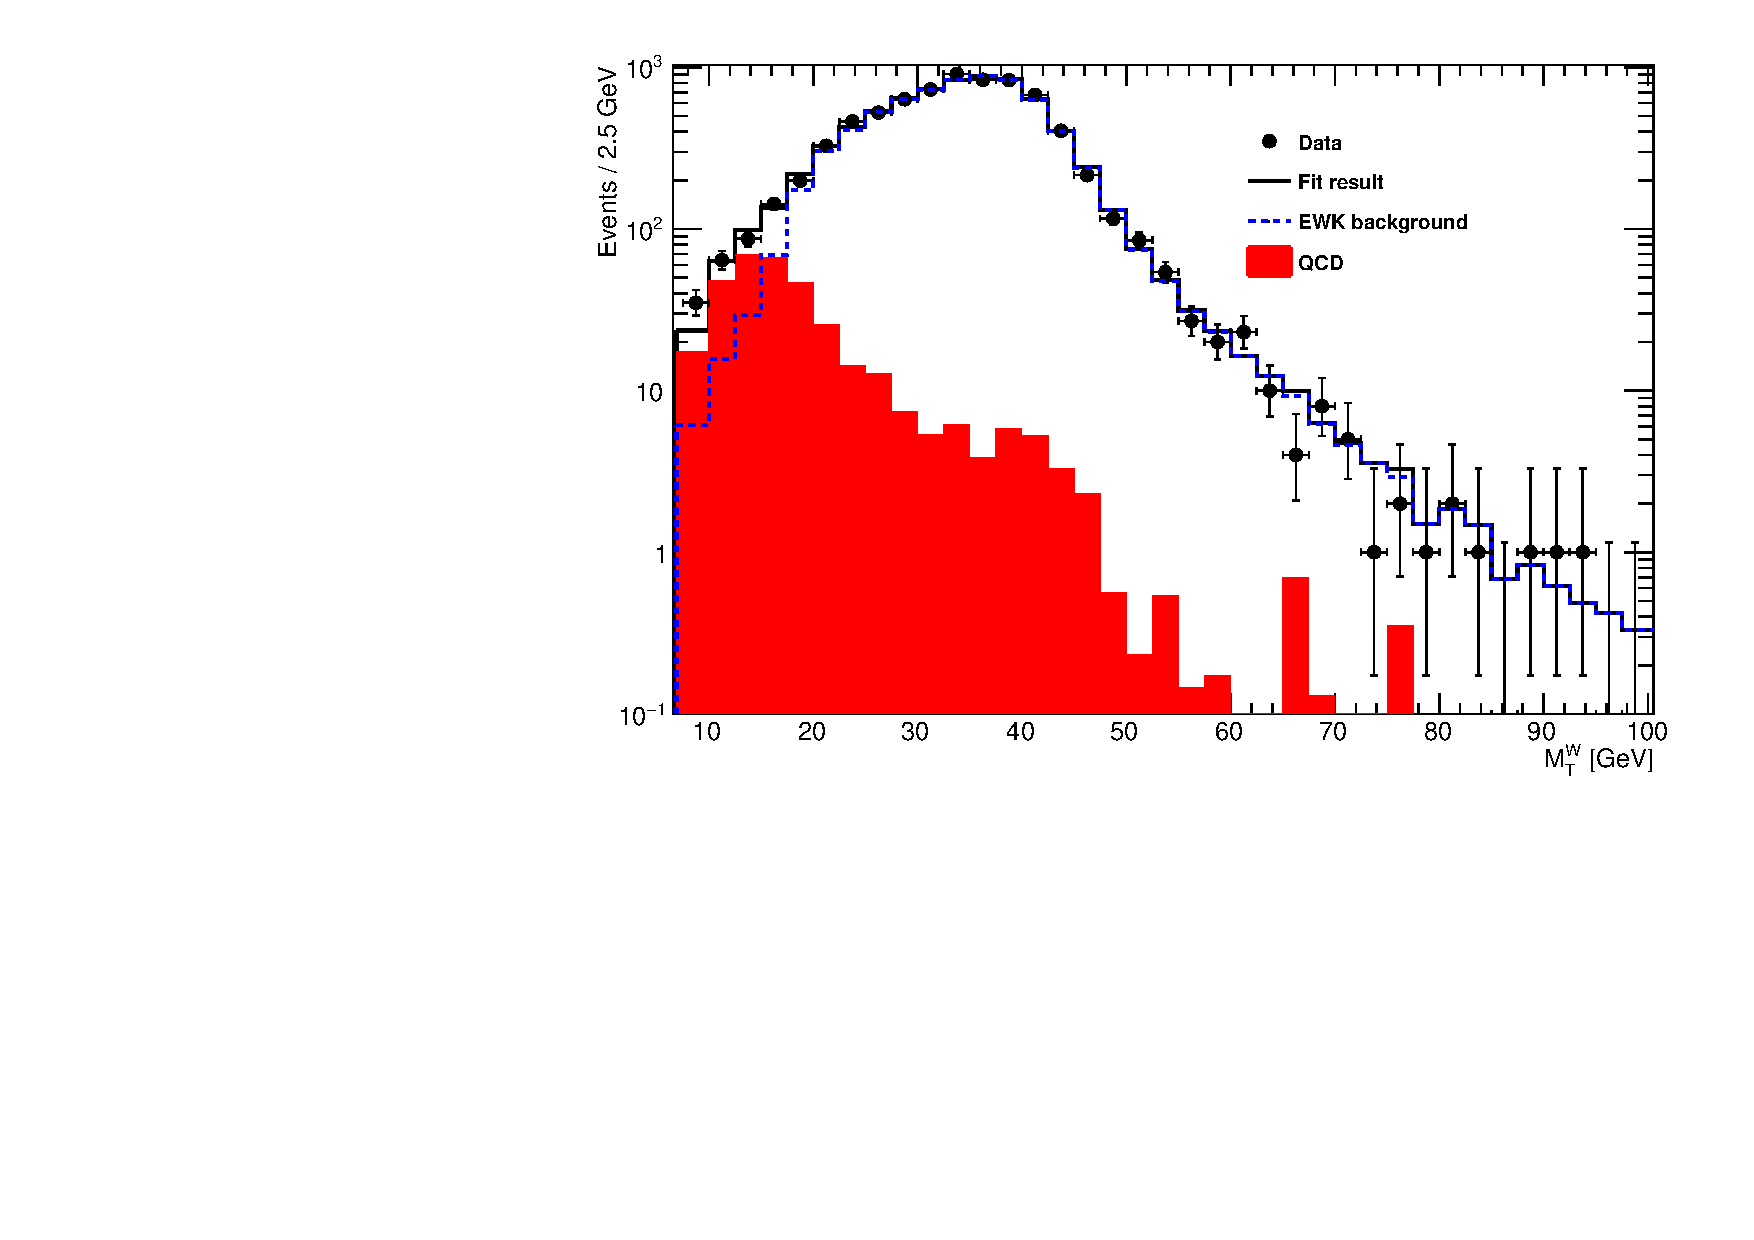
\includegraphics[width=1.\linewidth]{QCD/etMissFit.pdf} \\ a)}
\end{minipage}
\hfill
\begin{minipage}[h]{0.49\linewidth}
\center{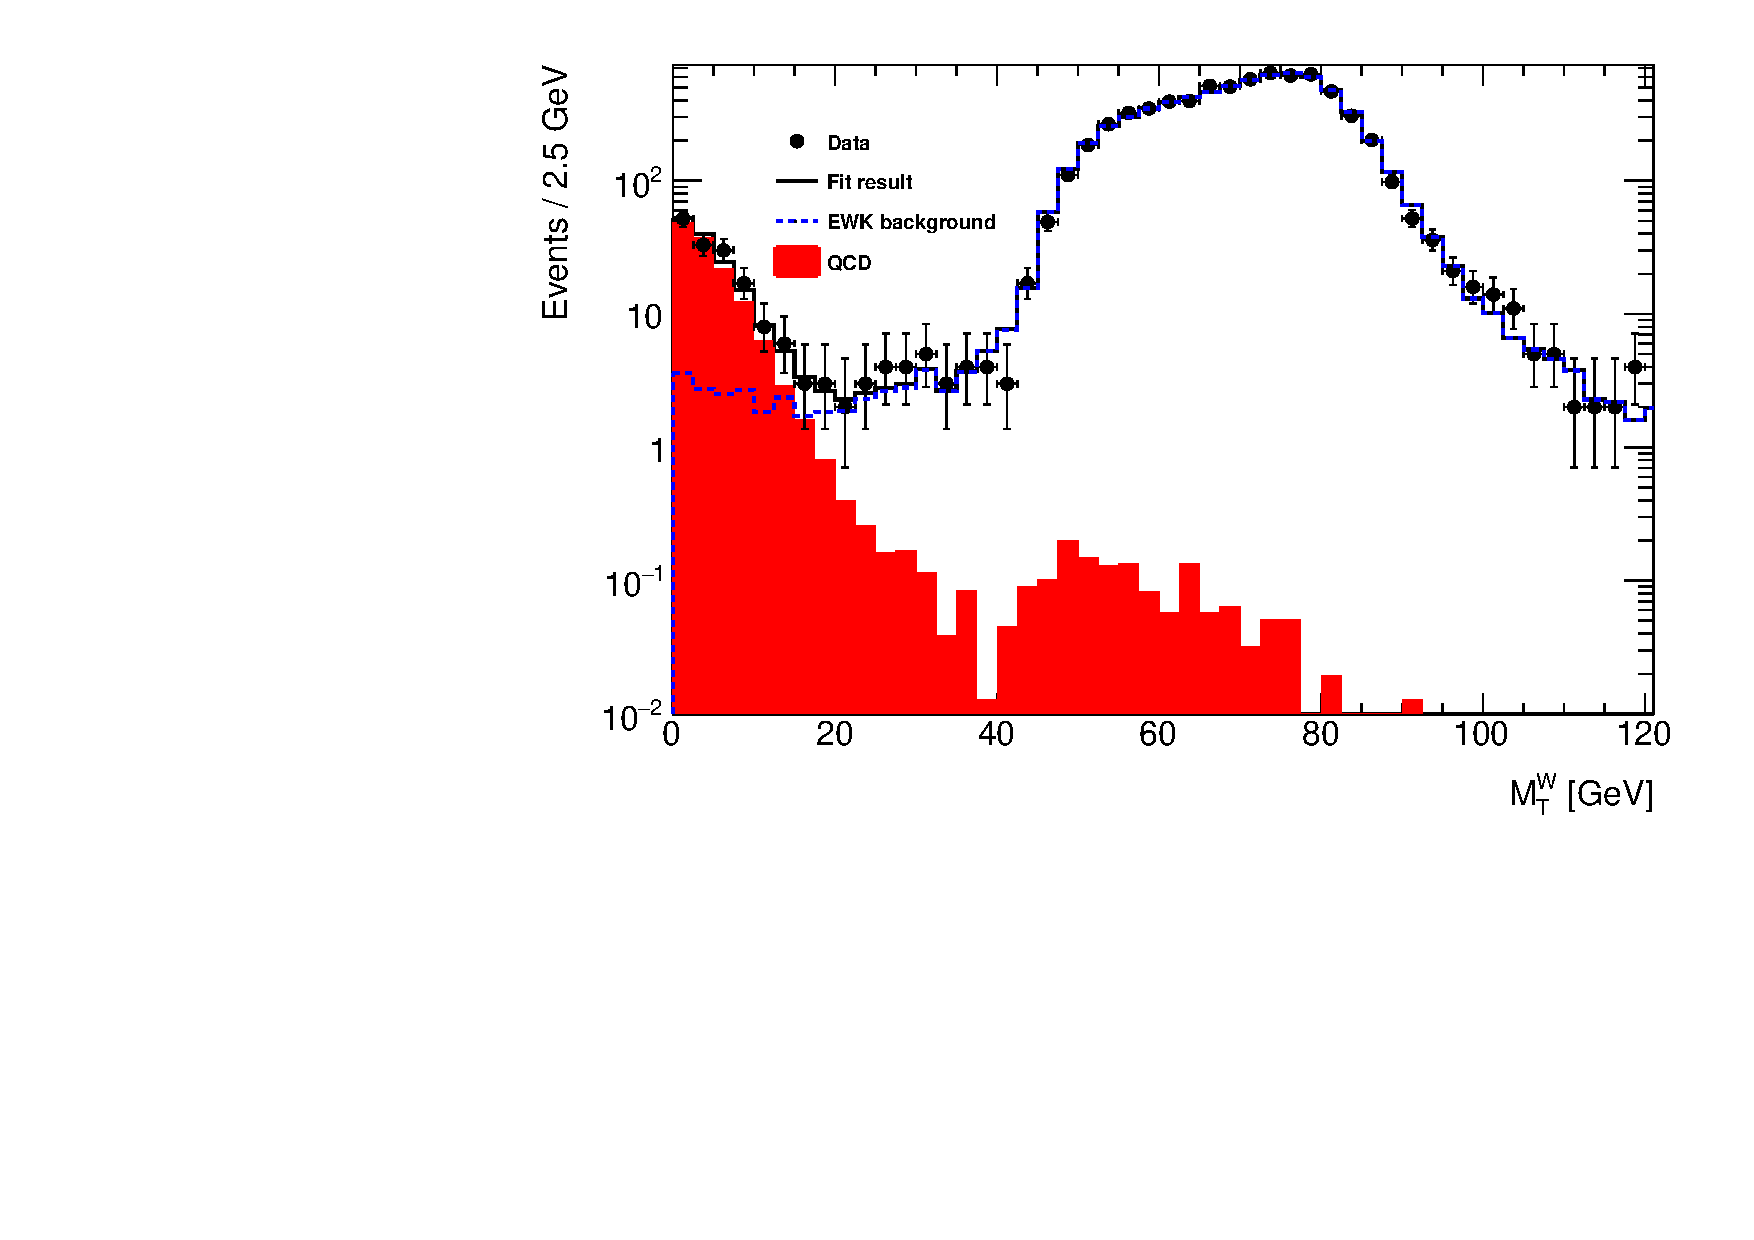
\includegraphics[width=1.\linewidth]{QCD/MtWFit.pdf} \\ b)}
\end{minipage}
\caption{The multijet background estimation for a) \wenu using reversed ID criteria and released \etmiss criteria b) \wmunu using released \mtw criteria and $b\bar{b}+c\bar{c}$ template.}
\label{ris:Fit}
\end{figure}

The normalization is found through the \chiD fit of the template and backgrounds to the data. The following composite model has been used for the estimation:
\begin{equation}
M(x) = \sum_{i=1}^{N-1}f_iF_i(x) + (1- \sum_{i=1}^{N-1} f_i)\cdot F_{QCD}(x),
\end{equation}
where index i goes over the MC samples, $x$ is a fit variable (\etmiss or \mtw), $F_i(x)$ and $ F_{QCD}(x)$ are the probability density functions of MC samples and multijet background template respectively. Fit parameters $f_i$ are the fractions of MC events within the fit region. In order to eliminate systematics, coming from the cross section uncertainty, the signal fractions are left as free parameters of the fit and the background MC fractions are allowed to be varied within 5\% uncertainty. 

Normalization scale of the multijet events is calculated from the obtained fit parameters as:
\begin{equation}
scale = \frac{(1-\sum f_i) \cdot N^{fit}_{Data}}{N_{template}},
\end{equation}
where $\sum f_i$ is a sum of all fractions in the fit, $N^{fit}_{Data}$ is a number of data events in a fit histogram and $N_{template}$ is a number of event in a template. The fit is performed separately for $W^{+}$ and $W^{-}$. Additionally, fit in total $W$ channel is used as a cross-check of the fit.
The results of the fitting procedure are shown in Fig.~\ref{ris:Fit} . 
 


\subsection{Systematic uncertainties estimation }\label{sec:QCDUnc}

\begin{figure}[!tbp]
\begin{minipage}[h]{0.49\linewidth}
\center{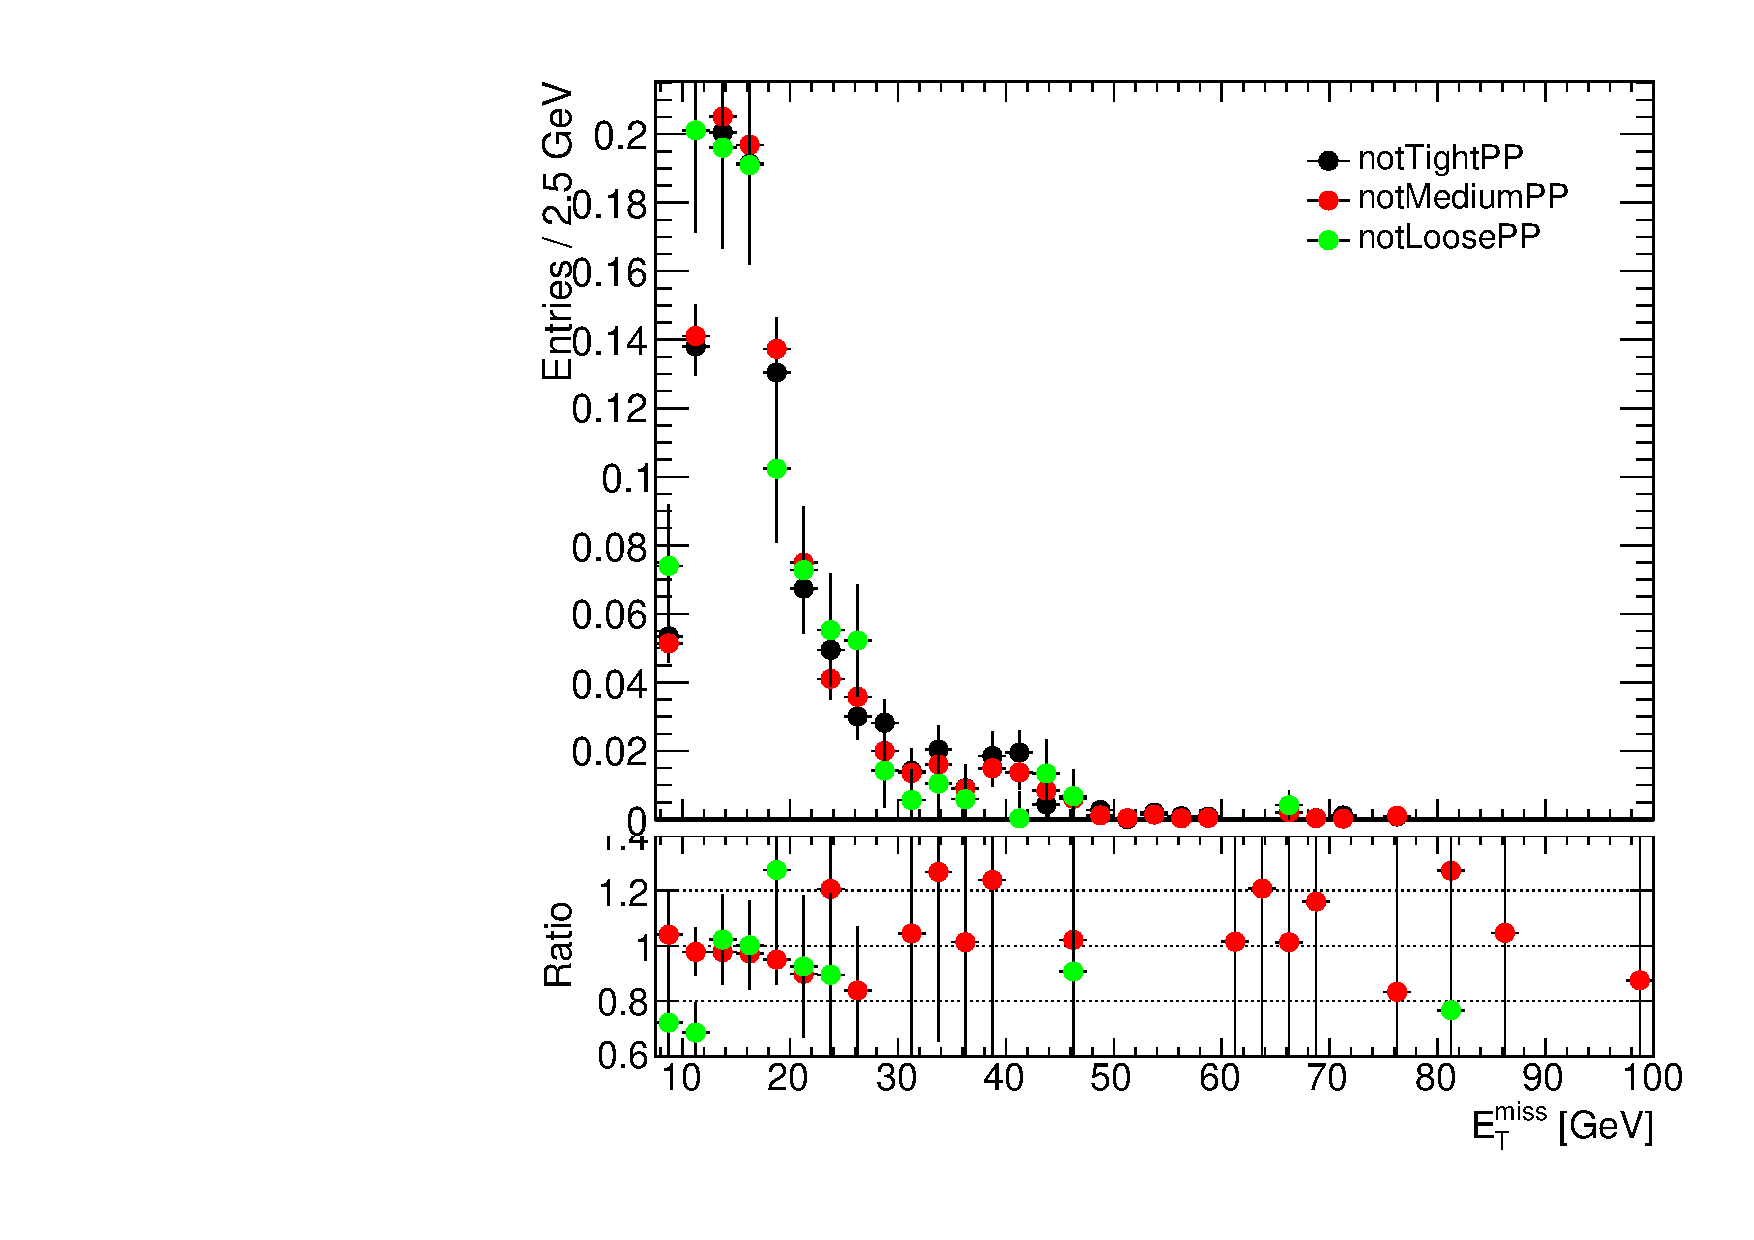
\includegraphics[width=1.\linewidth]{QCD/ElecTemplates.pdf} \\ a)}
\end{minipage}
\hfill
\begin{minipage}[h]{0.49\linewidth}
\center{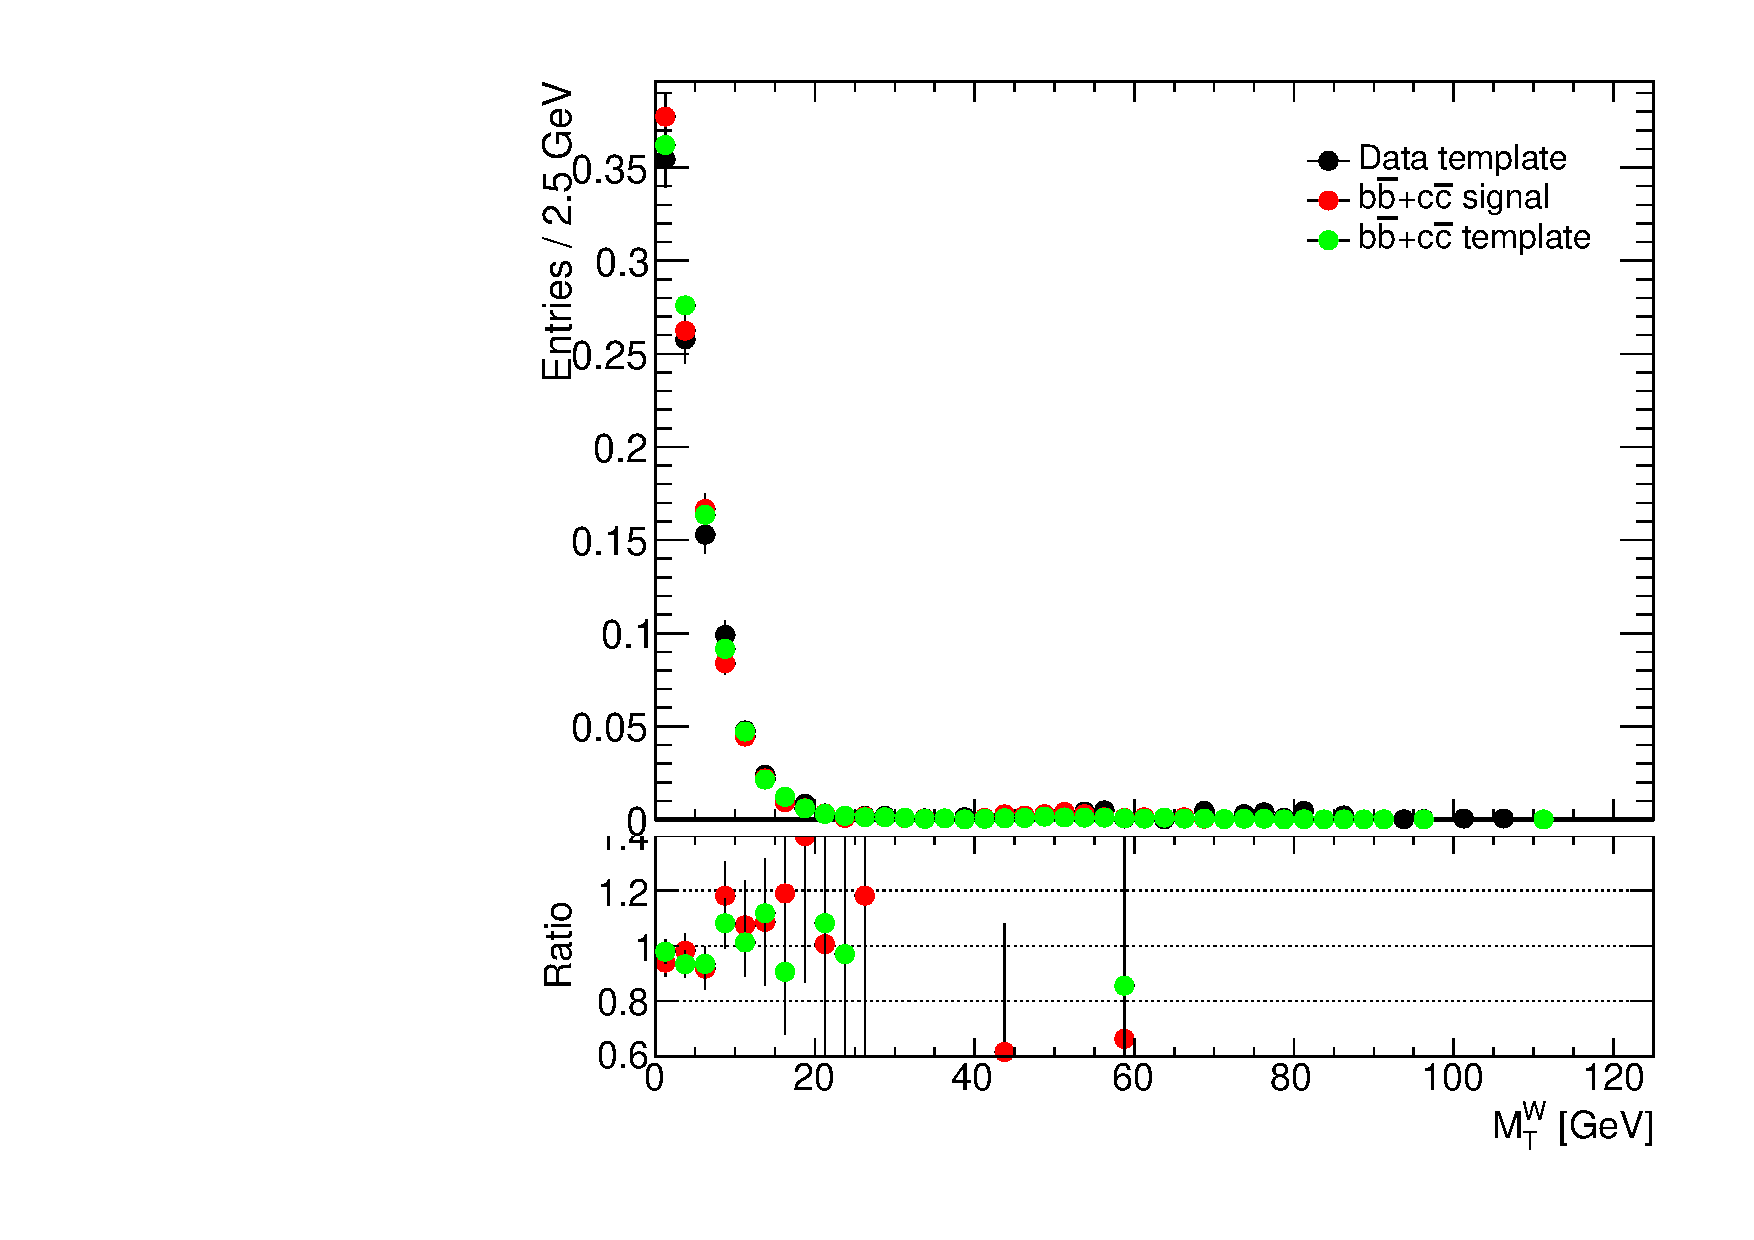
\includegraphics[width=1.\linewidth]{QCD/QCDBkgWmuTemplates.pdf} \\ b)}
\end{minipage}
\caption{The different QCD template comparison for a) \wenu and b) \wmunu analyses.}
\label{ris:TemplateVar}
\end{figure}

The uncertainty of the multijet background estimation can be divided into 3 main components:
\begin{equation}
\delta_{QCD} = \sqrt{ \delta_{fit\, unc}^{2}+\delta_{MC}^{2}+\delta_{fit\, bias}^{2}+\delta_{template}^{2}}, 
\end{equation}
where $\delta_{fit\, unc}$ is the uncertainty of a scale from a \chiD fit. The meaning of other components is explained below

The second component $\delta_{MC}$ is coming from a possible mismodelling of MC in a fitted region. It can be estimated by comparison of the fit results for $W$, $W^{+}$ and $W^{-}$. Number of multijet background events should not depend on a charge of W boson in the analysis, so it is expected:
\begin{equation}
N_{QCD}^{W^{+}}=0.5 \cdot N_{QCD}^{W} =N_{QCD}^{W^{-}}.
\end{equation}
Standard deviation of these 3 numbers is taken as systematic uncertainty. Since in \wmunu channel the multijet template normalization is derived from the fit at the small \mtw region, where electroweak contributions are negligible and the data statistics is high, this systematic source is equal to 0.



The third component $\delta_{fit\, bias}$ is coming from an effect of an arbitrary choice of bin size . This error is estimated by repeating the fit for different binnings. This component is assumed negligible in \wmunu case. 

The uncertainty $\delta_{template}$ is due to a potential bias in the template as a result of the template choice and a template statistics itself. For estimation of this uncertainty different template selections have been used. For \wenu channel different reversed isolation criteria have been tried (Fig.~\ref{ris:TemplateVar} a). The overall discrepancies can be considered negligible. For \wmunu channel template variations are estimated using fits with $b\bar{b}+c\bar{c}$ MC samples.  Fig.~\ref{ris:TemplateVar} b) compares data template with template obtained using signal selection with released \mtw requirement and template selection. Results for a different template fits are presented in Tab~\ref{tab:QCDWmunu}

\begin{table}[!tbp]
    \caption{Results of multijet background estimation for \wenu and corresponding error.}
	\label{tab:QCDWenu}
	\begin{center}
		\begin{tabular}{l | c | c | c | c }
		\hline
		    Charge & $N_{QCD}$ & $ \delta N_{fit\, unc} $ & $\delta N_{MC}$ & $\delta N_{fit\, bias}$ \\
		    \hline
		    $W^{+}$ & 38.3 & 7.0 & 7.0 & 5.0 \\
		    $W^{-} $ & 21.5 & 0.7 &  -9.4 & 4.0 \\
		    $W$ & 66.1 & 21.2 & 4.2 & 10.  \\
		    \hline
		    \hline
		    Total & 31.0 & 6.1 & 8.6 & 4.7 \\
		    \hline
		\end{tabular}
	\end{center}
\end{table}

\begin{table}[!tbp]
    \caption{Results of multijet background estimation for \wmunu using different templates and its fit error.}
	\label{tab:QCDWmunu}
	\begin{center}
		\begin{tabular}{l | c | c | c  }
		\hline
		    Charge & $N_{QCD}$ & $N_{QCD}$ & $N_{QCD}$ \\
		    & data template & $b\bar{b}+c\bar{c}$ template selection & $b\bar{b}+c\bar{c}$ signal selection \\
		    \hline
		    $W^{+}$ & 2.48 & 0.73 & 1.34 \\
		    $W^{-} $ & 2.48 & 0.73 & 1.35 \\
		    $W$ & 4.97 & 1.47 & 2.70  \\
		    \hline
		    \hline
		    Total per channel & 2.48 & 0.73 & 1.35 \\
		    Fit error & 0.60 & 0.73 & 0.19 \\
		    \hline
		\end{tabular}
	\end{center}
\end{table}


Results of the multijet background uncertainty estimation for \wenu and \wmunu are shown in Tab.~\ref{tab:QCDWenu} and~\ref{tab:QCDWmunu} respectively. The overall number of multijet background events is estimated as \nQCDWplusenu\,  for $W^{+}\to e^{+}\nu$ and $W^{-}\to e^{-}\nu$ and \nQCDWplusmunu\,   for $W^{+}\to \mu^{+}\nu$ and $W^{-}\to \mu^{-}\nu$. The overall fraction of the multijet events is lower, than in 13 TeV \cite{a13TeV} and 7 TeV \cite{a7TeV} data, what is in agreement with expectations.



\section{Background-subtracted W and Z boson candidate events}

Tab.~\ref{tab:BkgWlnu} summarizes the number of background events for W and Z selections. Uncertainties on a number of EWK+top events are coming from statistics, cross section uncertainty (if given) and 3.1\% of luminosity determination uncertainty. The multijet background uncertainty is esimtated in Sec.~\ref{sec:QCDUnc}. For the background-subtracted events the statistical uncertainty is quoted first, followed by the total systematic uncertainty, derived from the EWK+top and multijet backgrounds ones, considering the sources as uncorrelated. 



\begin{table}[!h]
    \caption{Number of observed candidate events for the $W \to l\nu$ channel, electroweak (EWK) and top, and data-driven multijet background events, and background-subtracted signal events.}
	\label{tab:BkgWlnu}
	\begin{center}
		\begin{tabular}{l || c || c | c || c  }
		\hline
		l & Observed & Background & Background & Background-subtracted \\
		 & candidates & (EWK + top) & (Multijet) & data $N_{W}^{sig}$ \\
		 \hline
		 \hline
		 & \multicolumn{4}{c}{W boson}\\
		 \hline
		 $e^{+}$ & \ntotWplusenu & \nEWttbarbkgWplusenu & \nQCDWplusenu & \ntotsignalWplusenu \\
		 $e^{-}$ & \ntotWminenu & \nEWttbarbkgWminenu & \nQCDWminenu & \ntotsignalWminenu \\
		 $\mu^{+}$ & \ntotWplusmunu & \nEWttbarbkgWplusmunu & \nQCDWplusmunu & \ntotsignalWplusmunu \\
		 $\mu^{-}$ & \ntotWminmunu &\nEWttbarbkgWminmunu & \nQCDWminmunu & \ntotsignalWminmunu \\
		 \hline
		 \hline
		 & \multicolumn{4}{c}{Z boson}\\
		 \hline
		 $e$ & \ntotZee & \nEWttbarbkgZee  & - &\ntotsignalZee \\
		 $\mu$ & \ntotZmumu &\nEWttbarbkgZmumu  & - & \ntotsignalZmumu \\
		 \hline
		 \end{tabular}
   \end{center}
\end{table}

